\subsection{Collateral Management Challenges}
\label{subsec:collateral_mgmt}
The collateral management process is currently tainted by several challenges, spanning various stages of the lifecycle and posing significant impediments to the efficient operation of financial markets. ISDA provides a breakdown of the most significant elements of friction in the process in their \textit{Blueprint for the Optimal Future State of Collateral Processing} \cite{isda_blueprint_collateral_processing} whitepaper (Figure \ref{fig:collateral_mgmt_steps}). These can be broadly categorised in the following areas:

\begin{itemize}
    \item \textbf{Asset Selection}. The process of asset selection, which determines what constitutes eligible collateral, is guided by a combination of regulatory stipulations and market conventions. However, the ultimate decision on what will be deemed eligible collateral is left to the discretion of the trading partners. This lack of standardization presents a significant challenge. The free-form nature of eligible collateral, typically defined in a Credit Support Annex (CSA), further compounds this issue. Moreover, difficulties arise in determining common definitions for certain asset types, such as high-quality liquid assets (HQLAs) \citep{HQLAs};

    \item \textbf{Margin and Interest Calculation}. The current process of margin and interest calculation is largely manual, making it prone to processing errors. Counterparties independently calculate their interest based on the terms of their agreements, which include agreed rates and day count. This independent calculation often leads to potential discrepancies thereby leading to settlement risk. The manual matching of interest calculation payments and the manual reconciliation process further exacerbate these challenges;

    \item \textbf{Trade Transaction Management}. Mismatched and unmatched trades are primary drivers of disputes in the margin and collateral process. High volumes of new trades and amendments result in daily volatility in portfolios, making the management of these trades a complex task. Portfolio reconciliation is managed on the day following execution, which limits the ability to resolve trade-matching issues prior to issuing margin calls.

    \item \textbf{Record Keeping and Reconciliation}. Record keeping and reconciliation are integral to the collateral lifecycle, but they are also time-consuming and costly. This fragmentation and the resulting inaccuracies pose significant challenges to the efficient operation of financial markets. For instance, the existence of up to 18 trade repositories (entities that centrally collects and maintains the records of OTC derivatives) globally, which are mostly regional or national, limits the scope of trades captured and hampers market transparency \citep{DTCC_trade_repositories}. These repositories are ill-equipped to offer the comprehensive data needed for policymakers to monitor and mitigate systemic risk effectively. As a result, the OTC derivatives market is likely to become less transparent in the future, further complicating record keeping and reconciliation efforts.

    \item \textbf{Operational Challenges}. The operational challenges associated with the collateral lifecycle are also significant. Principals often face difficulties in releasing assets as collateral due to regulatory rules and operational challenges. When certain assets are used as collateral, it involves physical movements of those assets to 3rd party accounts. This physical movement of assets incurs significant costs and operational overheads.

    \begin{figure}[!h]
        \centering
        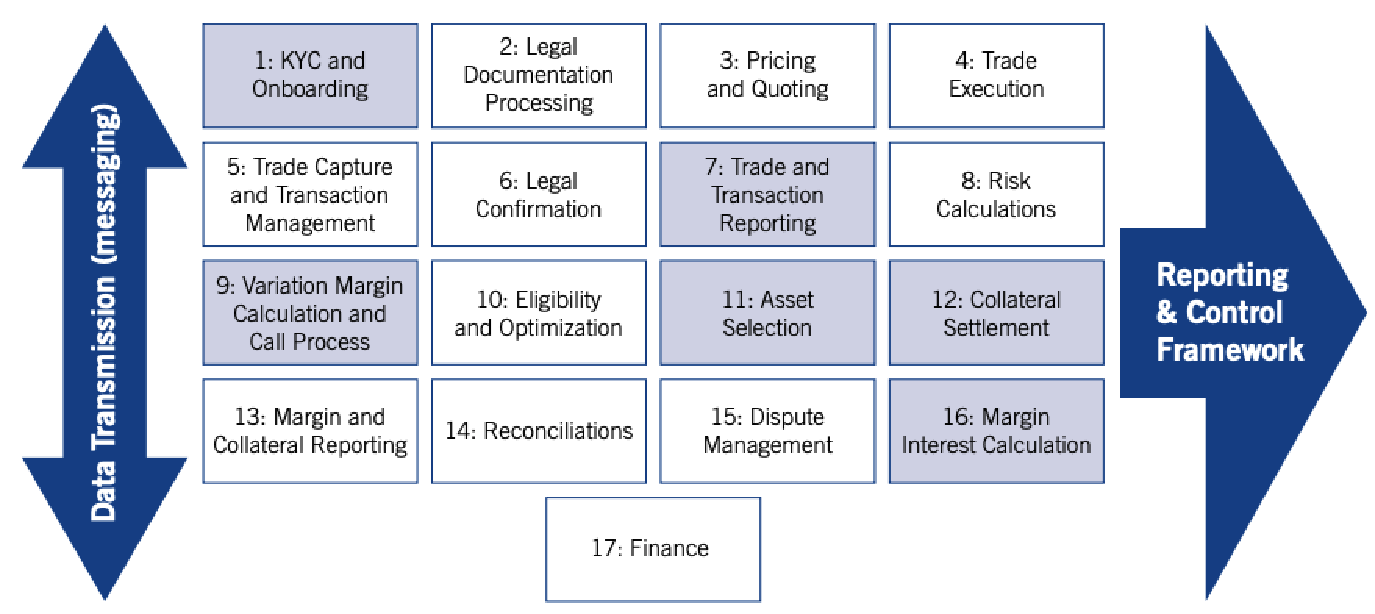
\includegraphics[width=\textwidth]{images/chapter-2/collateral-challenges.pdf}
        \caption[Collateral Management Processes]{Reproduced from \cite{isda_blueprint_collateral_processing}. Stages of Collateral Management: Highlighted steps are discussed in the ISDA Blueprint \citep{isda_blueprint_collateral_processing}. \textit{KYC \& Onboarding} often grapple with intricate due diligence requirements and data inconsistency across global jurisdictions. \textit{Trade and Transaction Reporting} faces the challenge of ensuring timely and accurate data submissions amidst diverse regulatory standards.\textit{ Variation Margin Calculation and Call Process} can be complex due to fluctuations in market prices and differing contractual terms. \textit{Asset Selection} confronts the dilemma of balancing optimal returns with counterparty acceptability and liquidity constraints.\textit{ Collateral Settlement} experiences delays due to multi-party involvement and reconciliation discrepancies. Lastly,\textit{ Margin Interest Calculation} struggles with diverse rate agreements and the intricacies of time-bound computations.}
        \label{fig:collateral_mgmt_steps}
    \end{figure}
    
\end{itemize}